\chapter{Design}

\begin{longtabu} to \linewidth{@{}l l l X[j]@{}}
    Version &    Dato &    Ansvarlig &    Beskrivelse\\[-1ex]
    \midrule
    1.0 &    15-04-2015 &    SSK &    Udkast til BDD, IBD\\
    1.1 &    23-04-2015 &    LSB og AJF &    Udkast for domænemodel og sekvensdiagrammer for hver UC\\
    1.2 &    27-04-2015 &    LSB og MFJ &    Udkast til klassediagrammer for hver UC. Grænseflader lavet. BDD færdig. IBD udeladt\\
    1.2 &   27-04-2015  &    SSK og MCM &    Påbegyndt UML-klassediagram\\
    2.0	&	29-04-2015	&	LSB, MFJ og AJF	&	Tilrettet domæne-, sekvens- og klassediagrammer, så design var klar til deadline\\
    2.1	&	12-05-2015	&	LSB, MFJ og AJF	&	Rettet design-dokument i forhold til kommentar fra vejleder\\
\label{version_Systemark}
\end{longtabu}

\section{Indledning}
Formålet med design afsnittet er at beskrive hardwaren og softwaren for EKG-systemet. Det beskrives vha.  diagrammer og skitser som tydeligør, hvordan de forskellige klassers funktionalitet er, og hvordan klasserne snakker sammen.
  
\section{Hardware arkitektur}
I dette projekt er hardwaren blevet udleveret, derfor vil hardware arkitekturen ikke blive beskrevet ned i mindste detalje, men derimod kun hardwarens overordnede funktion. Hardwaren for systemet består af en National Instruments DAQ og en signalgenerator fra Analog Discovery. Disse er begge forbundet til en computer via USB-porte.
\\ 
I dette projekt bliver EKG-signalet ikke målt fysisk via en patient, men simuleret via et signal, som er hentet ned fra websiden PhysioNet \footnote{http://www.physionet.org}. 

\begin{figure}[H]
	\centering
	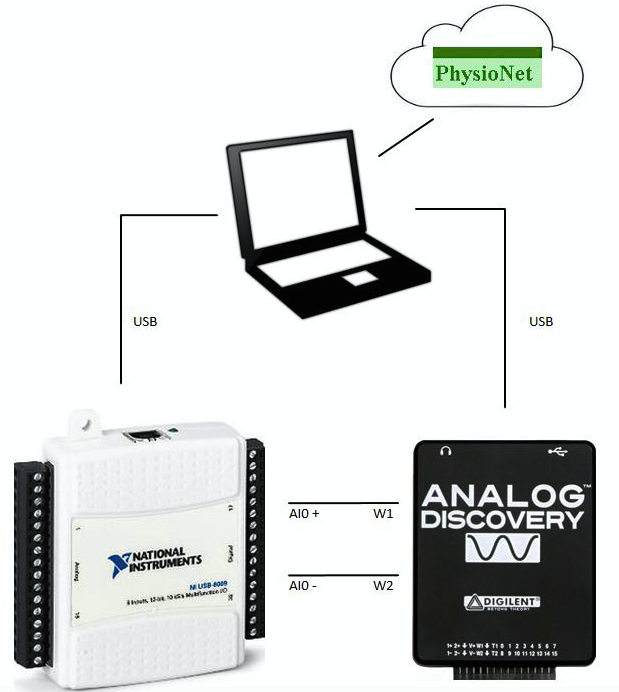
\includegraphics[width=0.6\textwidth]{Figurer/Snip20150427_1}
	\caption{Grafisk illustration af hardware opsætning}
\end{figure}

Som det ses på den overstående figur, er hardware opstillingen meget simpel. Figur 3.1 viser, hvordan de forskellige komponenter relaterer til hinanden. Display hardwaren vil i dette projekt være en computer, hvilket er et krav fra softwarens side, således at der kan vises et EKG-signal i form af en graf.
\\
\\  
Som beskrevet ovenfor er det Analog Discovery, som sammen med EKG-signalets informationer fra PhysioNet, der skaber den fiktive patient. Før EKG-signalet vises på computerens skærm, skal det igennem de forskellige komponenter i opstillingen. Analog Discovery modtager EKG-signalets  information som en CSV-fil, denne fil omdanner Analog Discovery til et analogt signal, som herefter sendes videre til DAQ’en. I DAQ’en digitaliseres det analoge signal, og tilpasses, så det efterfølgende kan udskrives på computer skærmen, i form af en EKG-graf. 

\subsection{Grænseflader}
Grænseflader af forbindelserne imellem de forskellige dele af hardwaren. 

\begin{table}[H] 
	\begin{tabularx}{\textwidth}{l l X}
    \toprule
     \textbf{Forbindelse}   & \textbf{Signaltype} & \textbf{Funktionalitet}    \\ \midrule
     DAQ - Computer         & Digital & DAQ'en konverterer det analoge signal til digitalt og videresender det til 							  computeren. Informationen sendes begge veje. \\ 
     					      \addlinespace[2mm]                                                                                                                                                                            
     Computer - Analog Discovery			& Digital & Computeren simulerer et EKG-signal og sender det til Analog Discovery.\\ 
     				    	  \addlinespace[2mm]   				                                                                                                                                                                           
     Analog Discovery - DAQ			   	& Analog & Analog Discovery	 konverterer signalet fra digitalt til analogt og videresender det til 							      DAQ'en.\\  				      
    \bottomrule                                                                                                                   
    \end{tabularx}
    \caption {Beskrivelse af grænseflader.}
    \label{tab:graenseflader}
\end{table}



\section{Software arkitektur}
I dette projekt arbejdes der med objektorienteret programmering i programmeringssproget C\#. Projektet er opbygget i henhold til trelagsmodellen. Præsentationslaget består af 4 GUI’er, logiklaget af en enkelt klasse, og datalaget består af 3 klasser, hvoraf den ene er en blackbox. 

\subsubsection{Trelagsmodellen}
Trelagsmodellen er en model, som kan bruges til at opbygge et system. Idéen er, at systemet opdeles i mindre moduler/lag - et præsentationslag (grænseflade), et logiklag (funktionalitet) og et datalag (database), som spiller sammen. \\
Præsentationslaget er det øverste lag. Det er det lag, brugeren har indvirkning på, og hvor de behandlede data præsenteres brugervenligt. \\
Logiklaget er det midterste lag. Dette lag er en slags bindeled mellem præsentationslaget og datalaget. I laget modtages og behandles informationerne fra præsentationslaget, og sendes videre til datalaget. Logiklaget kontrollerer hele systemets funktionalitet.\\
Datalaget er det nederste lag. Laget modtager dataerne fra logiklaget, som håndteres og lagres. Datalaget fungere som bindeled til databaser, hvor man kan gemme nye data og hente gamle data frem igen. Trelagsmodellen vil typisk bygges grafisk op som vist på nedenstående figur 3.2.\\

\begin{figure}[H]
	\centering
	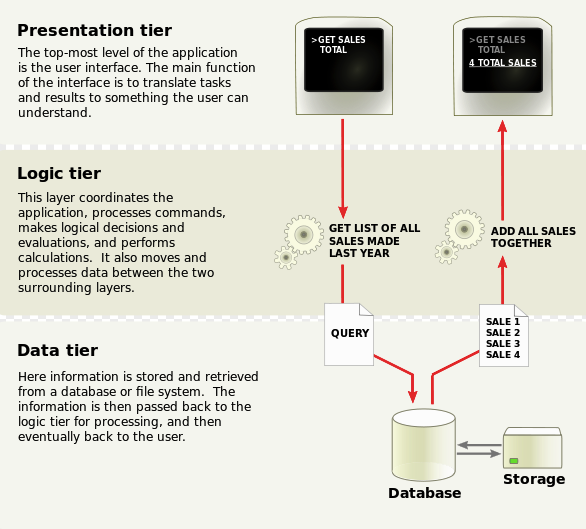
\includegraphics[width=1\textwidth]{Figurer/Snip20150415_39}
	\caption{Trelagsmodel\protect\footnotemark}
\end{figure}
\footnotetext{http://en.wikipedia.org/wiki/Multitier\_architecture}

Altså fungerer et system, opbygget efter trelagsmodellen, således, at alle lag er uafhængige af hinanden. Denne opbygning medfører, at systemet bliver mere overskueligt, samt det er muligt at forstå de enkelte lag hver for sig. At lagene er uafhængige er også en fordel, når der skal ændres i systemet. Det gør det muligt at begrænse vedligeholdelse til det aktuelle lag. Desuden er det muligt at modtage et lag fra et andet system, og ligeledes at sende og genbruge et lag andetsteds. I en projektgruppe er det også en fordel, at det er muligt at fordele arbejdet mellem gruppemedlemmer, og dermed kunne arbejde uafhængigt af andre.

\subsection{GUI}
I dette afsnit vil GUI’erne beskrives nærmere. Præsentationslaget består i alt af 4 GUI’er eller vinduer - Login-vindue, CPR-vindue, EKG-vindue og Gem\_måling-vindue.

\begin{figure}[H]
	\centering
	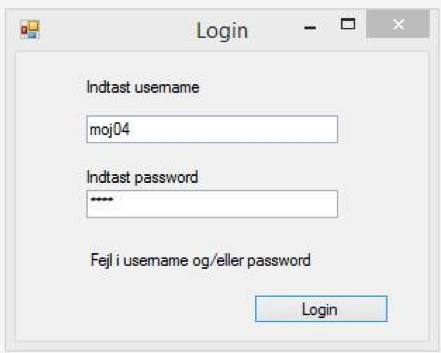
\includegraphics[width=0.8\textwidth]{Figurer/Snip20150430_38}
	\caption{Login-vindue}
\end{figure}

Når programmet startes op, vil et Login-vindue fremkomme på skærmen, se figur 3.3. Her skal brugeren logge ind for at få adgang til programmet, ved at indtaste sit personlige username og password. Bliver enten username eller password ikke godkendt, returneres en fejlmeddelelse, i form af en linje tekst nedenfor login-felterne. Bliver login godkendt åbnes CPR-vinduet, se figur 3.4.

\begin{figure}[H]
	\centering
	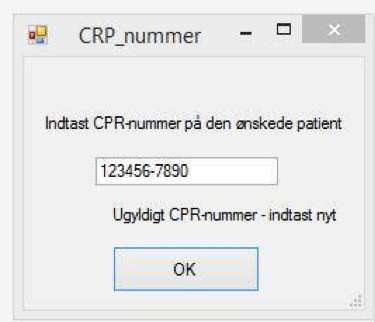
\includegraphics[width=0.6\textwidth]{Figurer/Snip20150430_39}
	\caption{CPR-vindue}
\end{figure} 

Her bliver brugeren bedt om at indskrive CPR-nummeret på den fiktive patient. CPR-nummeret bruges til at identificere personen i forbindelse med fremtidige målinger, samt til gemme målingerne i, hvad der svarer til den fiktive persons journal. Hvis CPR-nummeret ikke bliver godkendt, vil brugen blive gjort opmærksom på dette via en fejlmelding. 
\\
\\
Når CPR-nummeret bliver godkendt, åbner det primære vindue, EKG-vinduet, se figur 3.5. 

\begin{figure}[H]
	\centering
	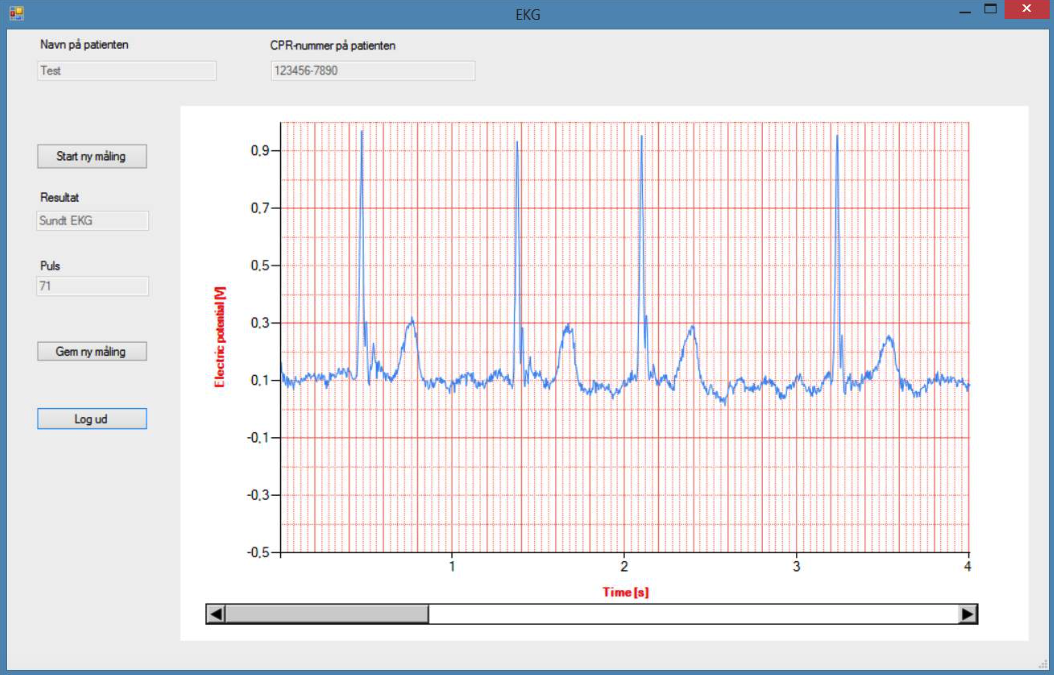
\includegraphics[width=1.0\textwidth]{Figurer/Snip20150525_25}
	\caption{EKG-vindue}
\end{figure}

EKG-vinduet er der, hvor man kan starte og se målinger. Vinduet er udstyret med knapper. Til højre i vinduet vises grafen over EKG-signalet, kort efter der er trykket ”Start ny måling”. Yderligere til venstre kan der i tekstboksen, ses puls for den pågældende graf. Under knappen "Start ny måling", vil diagnosen for EKG-signalet udskrives. Nederst til venstre i vinduet er der knapper til at gemme målingerne, samt at logge ud fra programmet. Desuden er der en scroller, der gør det muligt at se et større udsnit af EKG-signalet. Hvis man logger ud, kommer man tilbage til Login-vinduet, og EKG-vinduet er ikke længere synligt. 
\\
\\
Det sidste vindue, der er valgbart frembringes, når der trykkes på ”Gem ny måling”. Herefter vises pop-up vindue, som bekræfter, at den pågældende EKG-målingen er gemt, se figur 3.6. 

\begin{figure}[H]
	\centering
	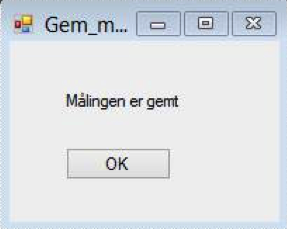
\includegraphics[width=0.5\textwidth]{Figurer/Snip20150430_41}
	\caption{Gem\_måling-vindue}
\end{figure}

\subsection{UML klassediagram}

\begin{figure}[H]
	\centering
	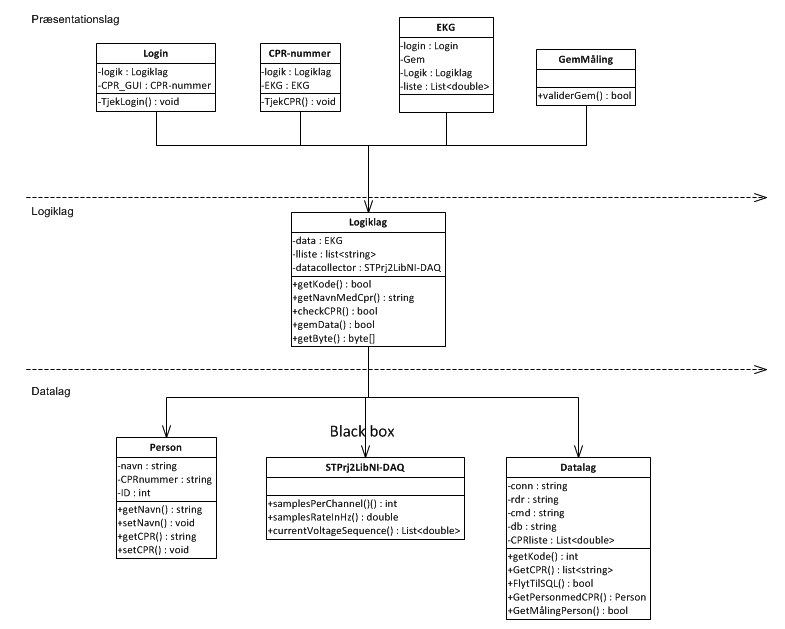
\includegraphics[width=1\textwidth]{Figurer/Snip20150512_9}
	\caption{UML-klassediagram over softwaren}
\end{figure}

Det ovenstående UML diagram (figur 3.7) over projektets software, giver en bedre og lettere forståelse for selve koden. Her er det meget tydeligt, at koden er opbygget efter trelagsmodellen. Præsentationslaget er bygget op af de førnævnte GUI’er, som bliver interfacen for selve bruger-interaktionen. I dette lag sker der som udgangspunkt intet behandlingsarbejde. Opsætningen og funktionerne af præsentationslaget er blevet yderligere beskrevet under afsnittet ’GUI’ 3.3.1.\\ \\
Logiklaget består af en enkelt klasse, der fungerer som programmets primære styring. Logiklaget er til for, at præsentationslaget ikke har direkte adgang til datalaget. Det er altså i dette lag, hvor alt programmets data bliver behandlet.  Her bliver EKG-siganlet f.eks. analyseret og login, samt CPR, bliver valideret i forhold til det data, der befinder sig i datalaget. \\ \\
Datalaget består af to klasser og en tilhørende blackbox. I det overstående er der kun beskrevet de metoder i blackboxen, som bliver brugt i andre klasser i programmet. I dette lag bliver der primært sørget for forbindelsen til databasen. Klassen ”Datalag” er kernen i dette lag. Her bliver der sørget for at gemme og hente informationer fra databasen. Det er i dette lag, hvor data som logiklaget arbejder med kommer fra. Klassen ”Person” er til for at binde alle person-informationer sammen, som medfører, at det kun er nødvendigt at kalde et enkelt objekt frem for 4 attributter. 

\subsection{Appliktationsmodel}
En standard applikationsmodel vil i almindelig forstand indeholde en overordnet domænemodel, herefter klassediagram samt sekvensdiagram og tilsidst et opdateret klassediagram, hvor metoderne fra sekvensdiagram er inkluderet. 

Applikationsmodellen for dette projekt består af en overordnet domænemodel, herefter sekvensdiagram for de forskellige Use Cases med tilhørende opdateret klassediagram, som beskriver metodekald og kommunikation mellem klasserne. Klassediagrammerne er her undladt, da de er irrelevante for dokumentationen af projektet. Applikationsmodellen er udarbejdet ud fra Use Cases, hvilket medfører, at metoderne er fiktive, altså ikke hentet direkte fra softwaren.  

\subsubsection{Domænemodel}
Domænemodellen er skabt på baggrund af de fem Use Cases. Gennem navneordsanalyse af Use Casene er de konceptuelle klasser fundet. I modellen beskrives, hvordan de konceptuelle klasser interagerer med hinanden. Controlleren er ikke en konceptuel klasse, men er den, der sørger for at systemet fungerer optimalt.

\begin{figure}[H]
	\centering
	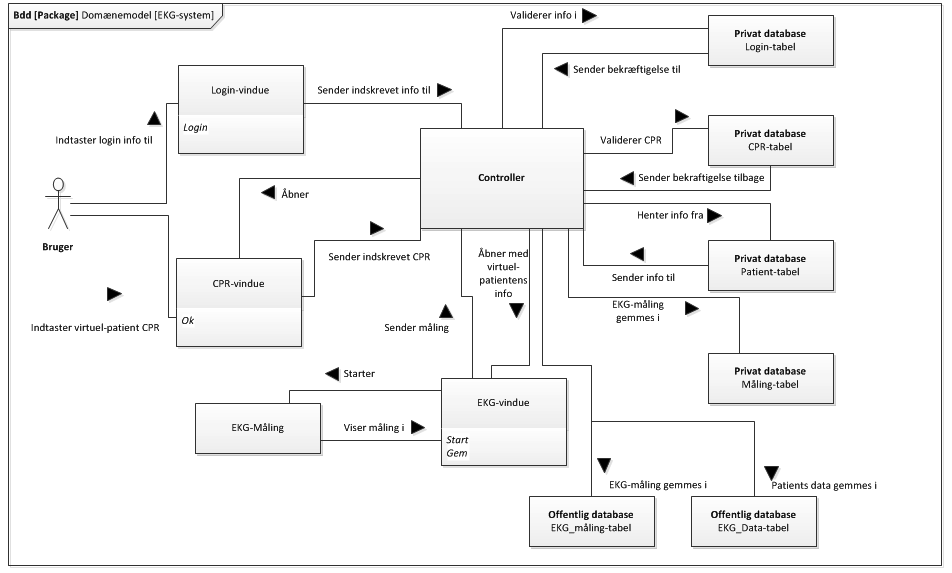
\includegraphics[width=1\textwidth]{Figurer/Snip20150525_18}
	\caption{Domænemodel af EKG-systemet}
\end{figure}

\subsubsection{Sekvensdiagram}
Sekvensdiagrammerne beskriver step-by-step, via fiktive metoder, forløbet i de forskellige Use Cases. Der er lavet et sekvensdiagram for hver Use Case, for at gøre systemet mere overskueligt. Et sekvensdiagram består af boundary-klasserne og domain-klasserne fra domænemodellen, samt en controller-klasse, med navn efter den specifikke Use Case.  

\begin{figure}[H]
	\centering
	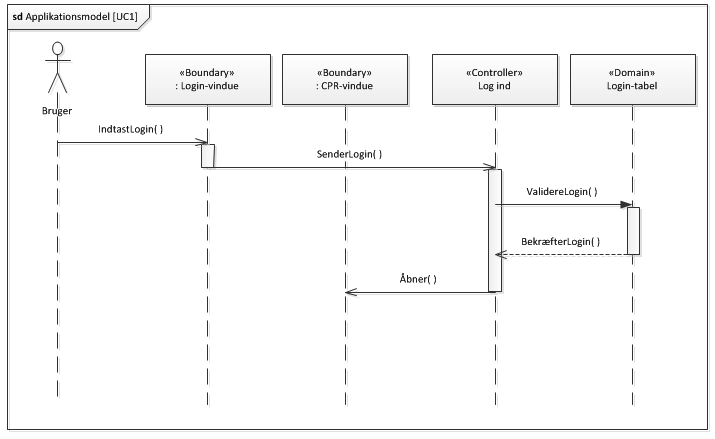
\includegraphics[width=0.9\textwidth]{Figurer/Snip20150429_34}
	\caption{Sekvensdiagram for UC1}
\end{figure}

\begin{figure}[H]
	\centering
	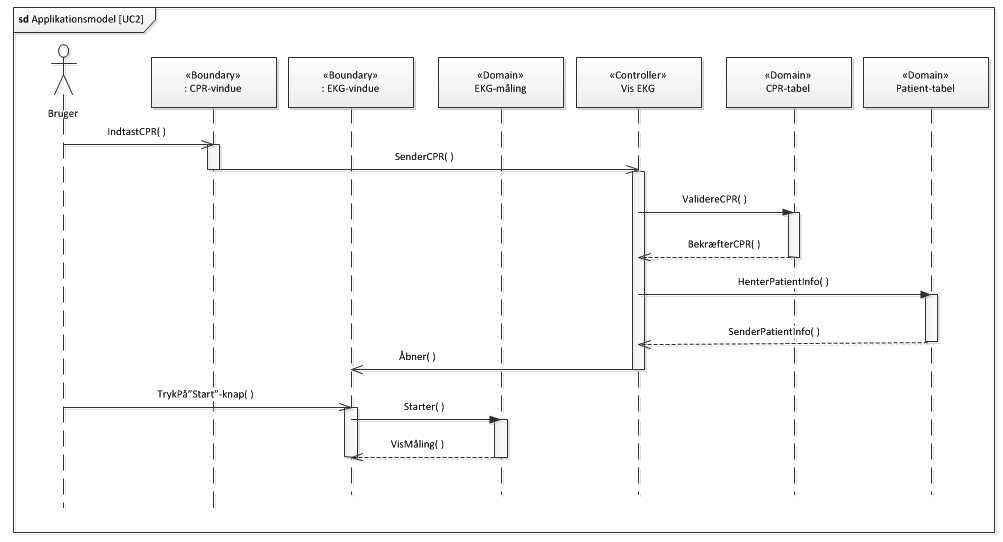
\includegraphics[width=1\textwidth]{Figurer/Snip20150429_33}
	\caption{Sekvensdiagram for UC2}
\end{figure}

\begin{figure}[H]
	\centering
	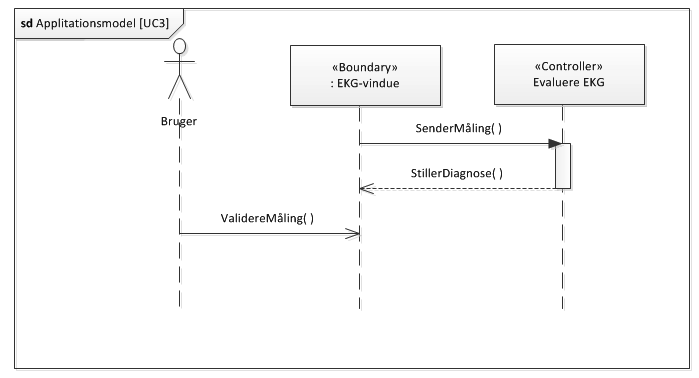
\includegraphics[width=1\textwidth]{Figurer/Snip20150429_31}
	\caption{Sekvensdiagram for UC3}
\end{figure}

\begin{figure}[H]
	\centering
	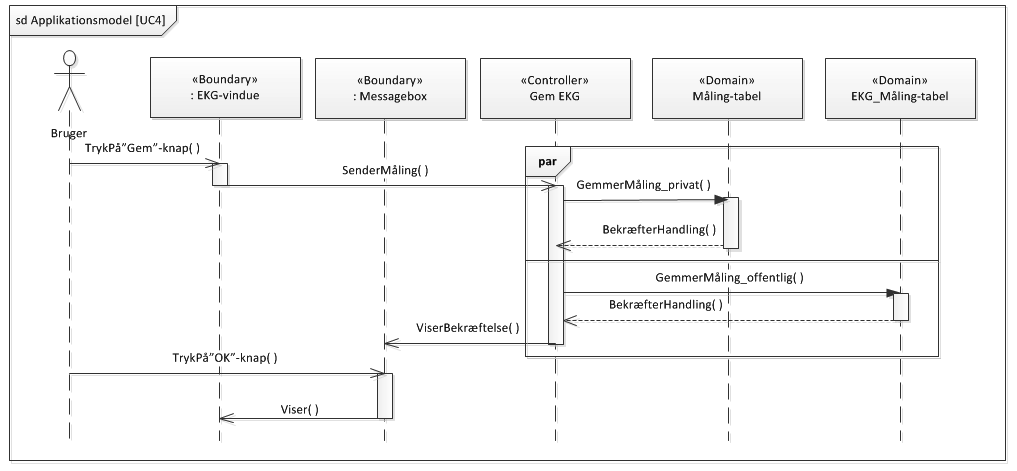
\includegraphics[width=1\textwidth]{Figurer/Snip20150525_21}
	\caption{Sekvensdiagram for UC4}
\end{figure}

\begin{figure}[H]
	\centering
	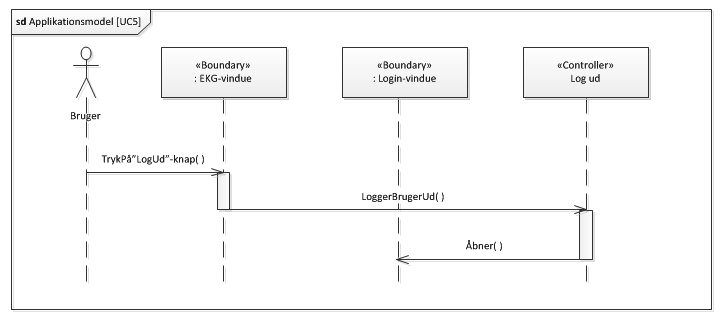
\includegraphics[width=1\textwidth]{Figurer/Snip20150429_30}
	\caption{Sekvensdiagram for UC5}
\end{figure}

\subsubsection{Opdateret Klassediagram}
De opdateret klassediagrammer indeholder metoderne fra de dertilhørende  sekvensdiagrammer - dette giver et overblik over, hvilke metoder de forskellige klasser består af.

\begin{figure}[H]
	\centering
	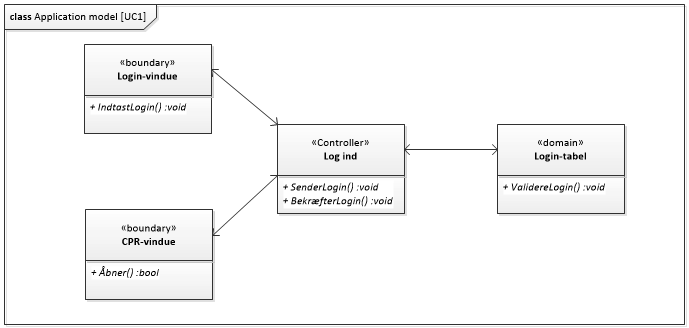
\includegraphics[width=1\textwidth]{Figurer/Snip20150429_20}
	\caption{Klassediagram for UC1}
\end{figure}  

\begin{figure}[H]
	\centering
	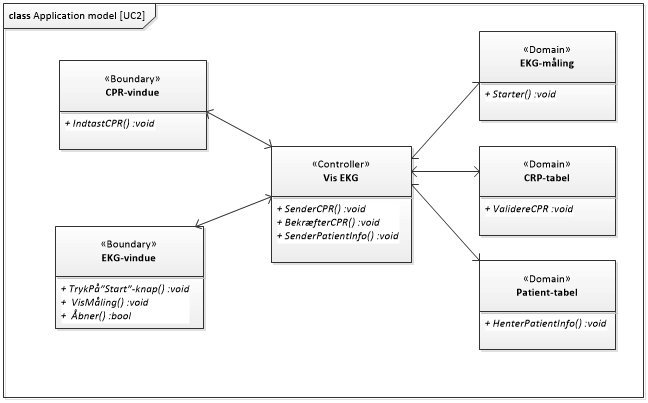
\includegraphics[width=1\textwidth]{Figurer/Snip20150429_22}
	\caption{Klassediagram for UC2}
\end{figure}

\begin{figure}[H]
	\centering
	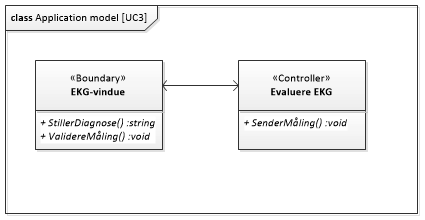
\includegraphics[width=0.8\textwidth]{Figurer/Snip20150429_23}
	\caption{Klassediagram for UC3}
\end{figure}

\begin{figure}[H]
	\centering
	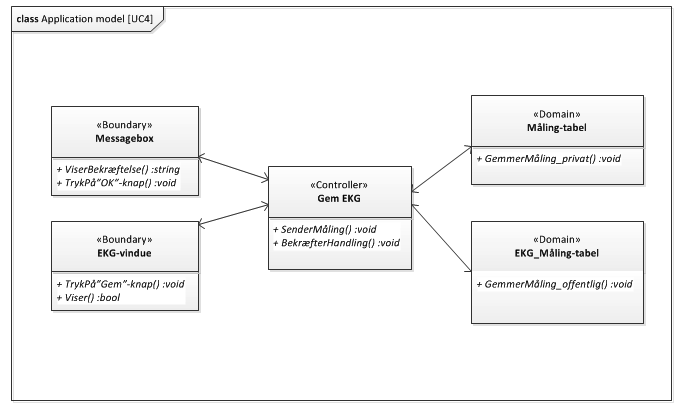
\includegraphics[width=1\textwidth]{Figurer/Snip20150525_20}
	\caption{Klassediagram for UC4}
\end{figure}

\begin{figure}[H]
	\centering
	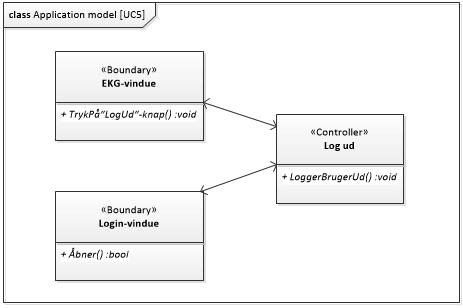
\includegraphics[width=1\textwidth]{Figurer/Snip20150429_25}
	\caption{Klassediagram for UC5}
\end{figure}

\section{Software implementering}
I dette afsnit vil ideen samt overvejelserne bag analysen af atrieflimren beskrives. Analysen fungere via et testprogram, som også her beskrives. Der vil være billeder, der understøtter og er forklarende til beskrivelsen. Kravene til programmet i forhold til at afbilde og gemme EKG-måling vil også i dette afsnit beskrives. 

\subsection{Visning af EKG-signal}
Grafen bliver genereret ved hjælp af en metode i logiklaget. Denne metode, "KørEKG", sætter de nødvendige forudsætninger for, at hardwaren bliver trigget til at starte en måling. Der bliver oprettet en ny sekvens, og herefter bliver navnet på enheden, samt den spænding, der kommer sat. Metoden returnerer herefter den måling, der bliver fortaget. \textbf{Henvisning}

\begin{figure}[H]
	\centering
	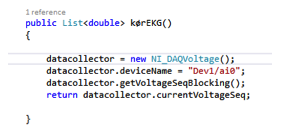
\includegraphics[width=0.8\textwidth]{Figurer/Snip20150525_39}
	\caption{Kode udsnit af visning af EKG-signal}
\end{figure}

Denne metode bliver efterfølgende kaldt i grafiklaget, nærmere betegnet i Formen EKG. \textbf{Henvisning}

\begin{figure}[H]
	\centering
	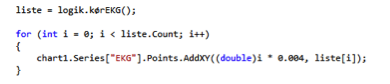
\includegraphics[width=1\textwidth]{Figurer/Snip20150525_40}
	\caption{Kode udsnit af visning af EKG-signal}
\end{figure}

Målingen bliver lagt over i en liste. Herefter køres alle punkter i målingen igennem, og bliver en for en lagt over i grafen. Disse bliver ganget med 0,004, for at konvertere samples til tid i sekunder. 


\subsection{Analyse}
Denne analyse er ikke bygget op omkring den grundlæggende definition af atrieflimren, altså at atrieflimren viser sig ved små fluktuationer på baselinen. Analysen er i stedet bygget op omkring informationen, om at amplituden i et bestemt frekvensområde vil være forhøjet, hvis der er mulighed for atrieflimren. \\ \\
Analysen af EKG’et består grundlæggende af tre for-løkker. \\ \\
Før analysen kan gå i gang, kræver det dog at den aktuelle EKG-sekvens bliver lavet om til et Furier-transformeret komplekst array. Her skal der bruges et bibliotek som indeholder metoder, som gør, at der kan bruges komplekst matematik i softwaren. Dette sker ved hjælp af en metode fra biblioteket alglibnet2. \\ \\
Herefter indeholder det komplekse array vektor-koordinator, som repræsenterer amplituden for alle frekvenser i signalet. I den første for-løkke, findes længden for alle vektorer en for en, og indsættes i listen amplitude. \\ \\
Da det er bevist, at atrieflimren viser sig ved forhøjet signalamplitude i frekvensspekteret 300 Hz til 400 Hz, er det der, softwaren skal tjekke om amplituden ligger over tærsklen. Før selve amplitudetærsklen kan vurderes, kræves det dog, at pladserne matchende frekvensspekteret, findes.\textbf{Omformuleres.} Måden de er fundet, er gjort rede for, i afsnittet omkring testprogrammet. \\ \\
I den næste løkke bliver de pladser, tilsvarende det valgte frekvensspektrum, lagt over i en liste for sig. Dette sker, fordi analysen kun er interesseret i de amplituder, som ligger i frekvensspektrummet, og det ville derfor være unødvendigt at kigge på samtlige 3600 amplituder, som er at finde i amplitude listen. Derfor ligges de udvalgte pladser i amplitudelisten over i endnu en liste, som indeholder de endelige amplitude-resultater for frekvensspektrummet i det aktuelle EKG-signal. \\ \\
Endelig bliver der i den sidste for-løkke vurderet om, hvorvidt amplituden i frekvensspekteret er højere end den valgte tærskel. \\ \\
Det skal nævnes, at denne analyse ikke passer på alle EKG-signaler. Dette er der to grunde til. Den ene er, at atrieflimren kan forme et signal på mange forskellige måder. Det vil derfor være svært at lave en analyse, som vil kunne dække over alle signaler. Den anden ting er, at alle mennesker er forskellige. Vores hjerterytmer kan have forskellige baselines, og vil derfor ligge forskelligt spændingsmæssigt. 

\subsection{Testprogram}
Den essentielle del i analysen er amplitudetærskelen. For at kunne vurdere tærsklen, kræver det, at man har værdier for både et rask og et sygt EKG, og ud fra dette vurderer, hvornår et signal har så betydelige ændringer i dets amplitude, at der kan være tale om atrieflimren. Til dette har gruppen valgt at skrive et testprogram. Programmet er skrevet og brugt i flere trin. Ligesom EKG-softwaren, er testprogrammet forbundet med matematik-biblioteket og STPrj2LibNI-DAQ-biblioteket. \\ \\
Fremgangsmetoden for behandling af signalet er i første omgang den samme som ved den reelle analyse; der laves en furier-transformation og derefter regnes arrayet om til en liste af amplituder. Ud over dette, laves der en liste af frekvenser. Dette sker ved dividere antal samples med antal pladser i arrayet, og derefter dividere resultatet med 2. Dette gøres for at fjerne fordoblingen af frekvenserne. \\ \\
De ønskede lister bliver herefter udskrevet i en tekstfil.


\begin{figure}[H]
	\centering
	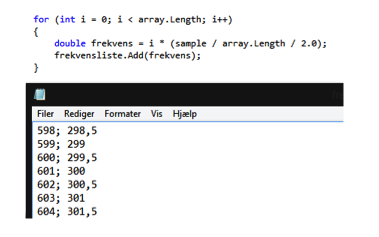
\includegraphics[width=1\textwidth]{Figurer/Snip20150520_12}
	\caption{Kode udsnit af testprogram}
\end{figure}

På figur (nummer \textbf{Sara skrive lige det selv.} ) kan der ses, hvor det valgte frekvensspekter ligger i listen. Herefter bekræftes det, at det valgte frekvensspekter, altså fra 300 Hz til 400 Hz, starter på plads 601 og slutter på plads 801. Derved skal der forstås, at amplituderne for frekvensspekteret altså også ligger på de samme pladser i deres liste. Herefter regnes længden af vektorerne ud, og disse bliver derefter også skrevet ud i en fil. Dette kan ses på figur (nummer \textbf{Sara skrive lige det selv.}). 


\begin{figure}[H]
	\centering
	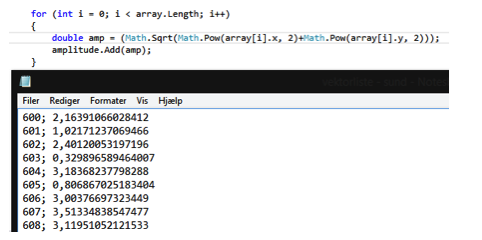
\includegraphics[width=1\textwidth]{Figurer/Snip20150520_13}
	\caption{Kode udsnit af testprogram}
\end{figure}

Det samme gøres for et sygt EKG. Herefter sammenlignes amplituderne, og der kan vurderes en tærskel. I vores projekt er tærsklen vurderet til at være 5.6 V. 

\subsection{Lagring i database}
Patienternes data og målinger gemmes i to forskellige databaser. Den ene database er oprettet af gruppen og den anden er en offentlige database udleveret af vejlederen i slutfasen af projektet. Den offentlige database bruges til at indrapportere EKG-målinger til brug til forskning og udveksling af EKG-målinger.  Der er brugt SQL til at gemme og hente patienternes data og EKG-målinger. Herunder vil der kort blive beskrevet hvordan SQL-koden er implementeret. 

\subsubsection{Offentlig database}
I den offentlige database findes der to tabeller med navnene EKG\_måling og EKG\_Data. Associationen mellem de to tabeller illustreres som følgende. Figur 3.23 viser, at en patient kan have mange EKG målinger. 

\begin{figure}[H]
	\centering
	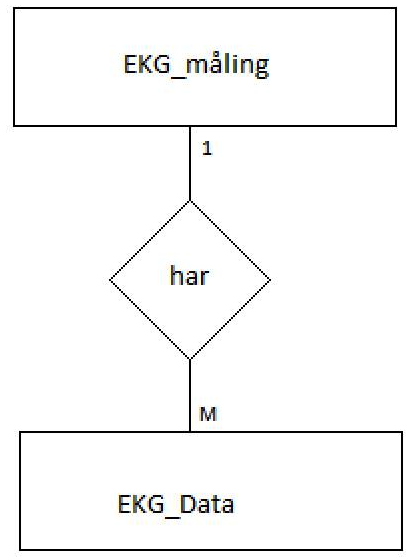
\includegraphics[width=0.4\textwidth]{Figurer/Snip20150525_38}
	\caption{Association mellem EKG\_måling og EKG\_Data}
\end{figure}

Opsætning til den offentlige database sker ved, at navnet til databasen erklæres vha. en private access specifier i datalaget. Herefter bruges en default constructor til at skabe forbindelse. Her fra er forbindelsen til den offentlige database skabt, se figur 3.24.

\begin{figure}[H]
	\centering
	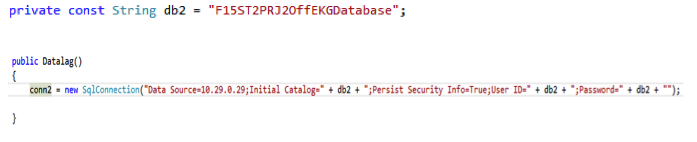
\includegraphics[width=1\textwidth]{Figurer/Snip20150525_32}	
	\caption{Kode udsnit fra lagring i database}
\end{figure}

Metoden "GemEKGDATA" gemmer patientens data i den offentlige database. De data som en patient har, kan ses som parametre i metoden. Disse data bliver lagt ind i de tilhørende kolonner i tabellen EKGDATA. Der er valgt én parameter til at demonstrere indsætning af en patients data i tabellen. De resterende parameter behandles tilsvarende. Se figur 3.25. 

\begin{figure}[H]
	\centering
	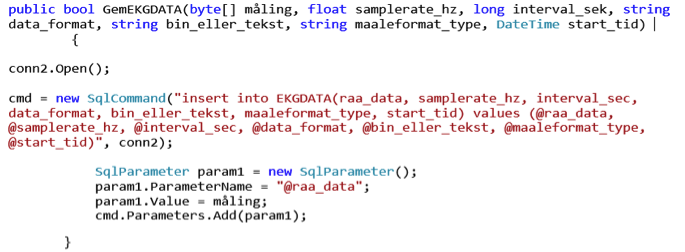
\includegraphics[width=1\textwidth]{Figurer/Snip20150525_33}
	\caption{Kode udsnit fra lagring af database}
\end{figure}

Tabellen EKGMAELING behandles på samme måde som tabellen EKGDATA. 

\subsubsection{Privat database}
Gruppens database indeholder tabellerne login, måling og patient. Indsættelsen af data er foretaget manuelt dvs. uden brug af SQL-kode. I figur 3.26 ses en skitse af patient-tabellen. 

\begin{figure}[H]
	\centering
	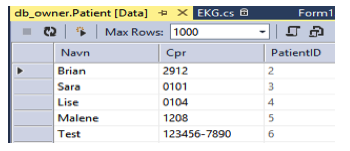
\includegraphics[width=0.8\textwidth]{Figurer/Snip20150525_34}
	\caption{Eksempel på tabel, Patient}
\end{figure}

Forbindelsen til denne databaseserver oprettes som tideligere eksempel, med den offentlige database, se figur 3.27.  

\begin{figure}[H]
	\centering
	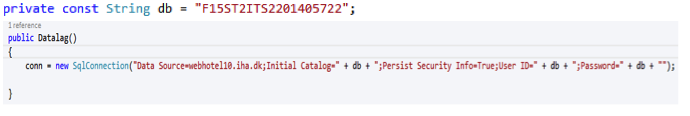
\includegraphics[width=1\textwidth]{Figurer/Snip20150525_35}
	\caption{Kode udsnit af privat databse}	
\end{figure}

SQL-koden i metoden "getKode" går ind tabellen "Login" og vælger en kode, som tilhører et bestemt navn. Hvis koden matcher det tilhørende navn, så returner den det ønskede navn og kode, se figur 3.28.   

\begin{figure}[H]
	\centering
	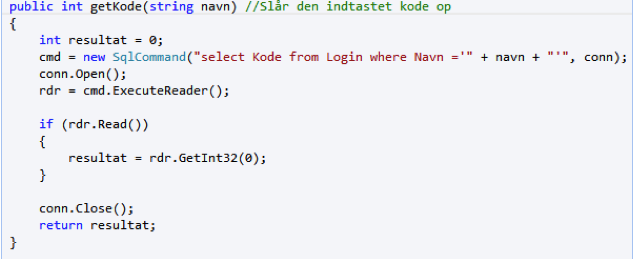
\includegraphics[width=1\textwidth]{Figurer/Snip20150525_36}
	\caption{Kode udsnit af privat database}
\end{figure}

De resterende SQL-koder for tabellen "patient" og "måling" i datalaget medtages ikke her, grundet deres sammenlignelighed med den overstående beskrivelse. Nærmere beskrivelse henvises til \textbf{hvor er det nærmere beskrevet, hvilket henvisning.} 









